%%%%%%%% ICML 2026 WORKSHOP — 4-PAGE SKETCH %%%%%%%%%%%%%%%%%

\documentclass{article}

\usepackage{microtype}
\usepackage{graphicx}
\usepackage{subcaption}
\usepackage{booktabs}
\usepackage{hyperref}
\usepackage{xcolor}
\usepackage{pgfplots}
\pgfplotsset{compat=1.18}
% Figure palette --- accessible, B&W-distinguishable, ICML-friendly.
\definecolor{plotScratch}{HTML}{6B6B6B}  % neutral dark gray (baseline)
\definecolor{plotIter1}{HTML}{2A6FAA}    % muted steel blue
\definecolor{plotIter2}{HTML}{D9690D}    % warm amber/orange (our result)
\definecolor{plotBand}{HTML}{F2F4F8}     % very light blue-gray band

\newcommand{\theHalgorithm}{\arabic{algorithm}}

\usepackage{icml2026}

\usepackage{amsmath}
\usepackage{amssymb}
\usepackage{mathtools}
\usepackage{amsthm}
\usepackage{algorithm}
\makeatletter
\let\algorithmic\relax
\let\endalgorithmic\relax
\makeatother
\usepackage{algpseudocode}

\usepackage[capitalize,noabbrev]{cleveref}

\theoremstyle{plain}
\newtheorem{theorem}{Theorem}[section]
\newtheorem{proposition}[theorem]{Proposition}
\newtheorem{lemma}[theorem]{Lemma}
\theoremstyle{definition}
\newtheorem{definition}[theorem]{Definition}

\usepackage[textsize=tiny]{todonotes}

\icmltitlerunning{Spectrogram-Only Self-Supervision for Low-Resource ASR}

\begin{document}

\twocolumn[
  \icmltitle{Spectrogram-Only \\
    Self-Supervised Pretraining for Low-Resource Speech Recognition}

  \icmlsetsymbol{equal}{*}

  \begin{icmlauthorlist}
    \icmlauthor{Anonymous Author}{yyy}
  \end{icmlauthorlist}

  \icmlaffiliation{yyy}{Anonymous Institution}

  \icmlcorrespondingauthor{Anonymous Author}{anon@anon.edu}

  \icmlkeywords{self-supervised learning, speech recognition, low-resource}

  \vskip 0.3in
]

\printAffiliationsAndNotice{}

\begin{abstract}
Automatic speech recognition (ASR) systems depend on large amounts of labeled data, a constraint that self-supervised pretraining (SSL) aims to alleviate. While existing SSL methods such as wav2vec~2.0 and HuBERT achieve state-of-the-art performance, they operate on raw waveforms and require thousands of GPU-hours of pretraining, making them impractical in compute-constrained and edge-deployment settings. In this paper, we reformulate self-supervised speech representation learning in the spectrogram domain, using a HuBERT-style masked-prediction objective over dual-codebook discrete units first derived from short log-mel chunks and then optionally refined from encoder representations. Applied to a 9M-parameter SqueezeFormer-XS encoder, our iter-2 recipe reduces test-clean WER from 71.3\% to \textbf{32.1\%} (39.2 absolute, \textbf{55\% relative}) when fine-tuned on 10 hours of labeled data, and from 21.5\% to 17.4\% (4.1 absolute, 19\% relative) on 100 hours --- at \emph{42 GPU-hours} of estimated pretraining, roughly $\mathbf{50\times}$ less reported GPU-hours than wav2vec~2.0 Base.
\end{abstract}

\begin{figure}[t!]
  \centering
  % --- DUMMY FIGURE: numbers are placeholders matching the iter-2 row
  % of Table~1. Replace the {x, y} pairs in each \addplot when final
  % results land. Keep the structure identical.
  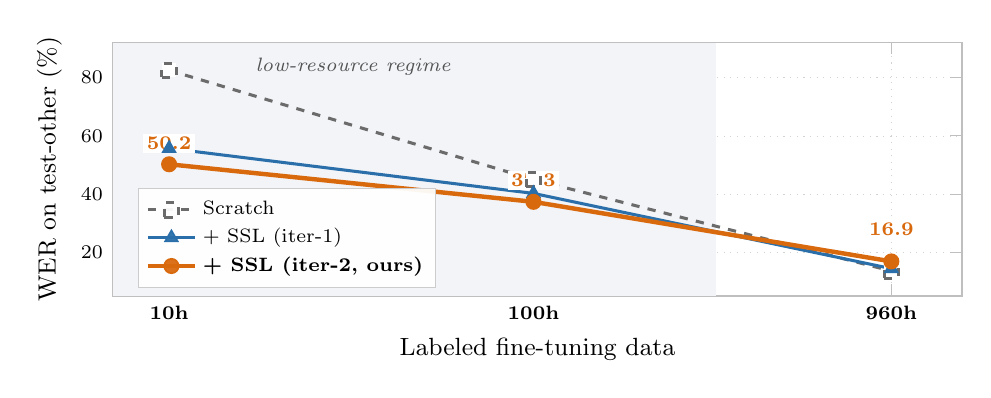
\begin{tikzpicture}
    \begin{semilogxaxis}[
        width=1.02\columnwidth,
        height=4.8cm,
        xlabel={Labeled fine-tuning data},
        ylabel={WER on test-other (\%)},
        xmin=7, xmax=1500,
        ymin=5, ymax=92,
        xtick={10,100,960},
        xticklabels={\textbf{10h}, \textbf{100h}, \textbf{960h}},
        ytick={20,40,60,80},
        grid=major,
        major grid style={dotted, line width=.15pt, draw=gray!35},
        axis line style={draw=gray!50},
        tick style={draw=gray!50},
        legend pos=south west,
        legend cell align=left,
        legend style={
          font=\scriptsize,
          draw=gray!40,
          fill=white,
          fill opacity=0.94,
          text opacity=1,
          row sep=-0.5pt,
          inner sep=2.5pt,
        },
        label style={font=\small},
        tick label style={font=\scriptsize},
        every axis plot/.append style={
          line width=1.1pt,
          mark size=2.6pt,
          mark options={solid, line width=0.6pt},
        },
        clip=false,
      ]

      % --- Shaded "low-resource regime" band ---
      \fill[plotBand] (axis cs:7,5) rectangle (axis cs:316,92);

      % --- Scratch baseline ---
      \addplot[color=plotScratch, dashed, mark=square*,
               mark options={fill=white, draw=plotScratch}]
        coordinates {(10, 82.48) (100, 44.96) (960, 13.57)};
      \addlegendentry{Scratch}

      % --- SSL iter-1 ---
      \addplot[color=plotIter1, mark=triangle*]
        coordinates {(10, 55.67) (100, 40.21) (960, 14.39)};
      \addlegendentry{+ SSL (iter-1)}

      % --- SSL iter-2 (ours) — highlighted ---
      \addplot[color=plotIter2, mark=*, line width=1.6pt]
        coordinates {(10, 50.21) (100, 37.32) (960, 16.86)};
      \addlegendentry{\textbf{+ SSL (iter-2, ours)}}

      % --- Inline data labels on the iter-2 line ---
      \node[font=\scriptsize\bfseries, plotIter2, fill=white, inner sep=1.2pt,
            anchor=south, yshift=4pt]
        at (axis cs:10,50.21)  {50.2};
      \node[font=\scriptsize\bfseries, plotIter2, fill=white, inner sep=1.2pt,
            anchor=south, yshift=4pt]
        at (axis cs:100,37.32) {37.3};
      \node[font=\scriptsize\bfseries, plotIter2, fill=white, inner sep=1.2pt,
            anchor=south, yshift=8pt]
        at (axis cs:960,16.86) {16.9};

      % --- Region annotation: italic label inside the shaded band, kept
      % well above any line via a large yshift so nothing overlaps.
      \node[font=\scriptsize\itshape, gray!65!black, anchor=north]
        at (axis cs:32,90) {low-resource regime};
    \end{semilogxaxis}
  \end{tikzpicture}
  \vskip -1ex
  \caption{Test-other WER vs.\ labeled fine-tuning data on LibriSpeech.
    Spectrogram-domain SSL delivers large absolute WER reductions in the
    low-resource regime (shaded band). At 960h, both SSL initializations
    underperform scratch under the current fine-tuning recipe.}
  \label{fig:wer-vs-hours}
\end{figure}

\section{Introduction \& Related Work}
\label{sec:intro}

Automatic Speech Recognition (ASR), commonly referred to as Speech-To-Text, is the task of converting spoken language into written text through computational methods. In recent years, end-to-end (E2E) neural networks have been scaled to near-perfect performance on standard benchmarks. Early end-to-end systems combined recurrent encoders with the connectionist temporal classification (CTC) loss~\citep{deepspeech}, replacing the modular HMM-GMM pipeline with a single trainable network. Subsequent work shifted to attention-based encoders: the Conformer~\citep{conformer} interleaves convolution and self-attention to capture both local and global acoustic structure, and remains a strong default backbone. More recent variants pursue efficiency without sacrificing accuracy --- for instance, HyperConformer~\citep{hyperconformer} replaces self-attention with hypernetwork-driven mixers, while SqueezeFormer~\citep{squeezeformer} redesigns the macro-architecture entirely. We adopt SqueezeFormer-XS as our backbone for its favorable accuracy--parameter trade-off in the compact regime.

A key limitation of these models, however, is their heavy dependence on labeled data, making them impractical in low-resource settings. Self-supervised pretraining on \emph{raw waveforms} has emerged as the dominant strategy to address this constraint. Early work such as vq-wav2vec~\citep{vqwav2vec} introduced discrete acoustic units via vector quantization, paving the way for masked-prediction objectives in the speech domain. Building on this, wav2vec~2.0~\citep{wav2vec2} learns contrastively over masked latent representations; HuBERT~\citep{hubert} replaces the contrastive target with prediction of offline-clustered units; WavLM~\citep{wavlm} extends this with denoising and speaker-mixing objectives; and data2vec~\citep{data2vec} unifies the masked-prediction recipe across modalities by regressing teacher-network targets. These methods reach state-of-the-art on LibriSpeech~\citep{librispeech} but rely on large transformer encoders and thousands of GPU-hours of pretraining on unlabeled audio, which is prohibitive in compact-model and edge-deployment settings.

A parallel line of work applies self-supervised learning directly to \emph{spectrograms} rather than raw waveforms. Masked Spectrogram Prediction~\citep{msp} and Audio Spectrogram Transformer (AST;~\citep{ast}) demonstrate that patch-based masked autoencoding over mel-spectrograms yields rich audio representations — however, these models are designed for general audio classification and are not directly applicable to the sequence-to-sequence demands of ASR. SSAST~\citep{ssast} bridges this gap by applying joint masked prediction and contrastive objectives over spectrogram patches in a self-supervised manner, yet remains anchored to large transformer backbones with substantial pretraining costs.

In this work, we present a spectrogram-domain SSL pipeline that combines log-mel chunk clustering with masked-prediction pretraining of a compact SqueezeFormer encoder. First-stage targets are produced by PCA-reduced $K$-means over short log-mel chunks at two granularities ($K_c{=}100$ coarse, $K_f{=}500$ fine). We additionally evaluate an optional second refinement stage in which targets are recomputed from the iter-1 encoder's hidden states. The recipe yields consistent WER improvements over from-scratch baselines in the 10h and 100h fine-tuning regimes at roughly $\mathbf{50\times}$ lower reported pretraining GPU-hours than wav2vec~2.0 Base, and we ablate the contribution of each codebook to validate the dual-vocabulary design.

\paragraph{Contributions.}
(i) A simple, teacher-free, spectrogram-domain SSL recipe that pretrains a 9M-parameter encoder in an estimated 42 GPU-hours --- about $50\times$ lower reported GPU-hours than wav2vec~2.0 Base.
(ii) A dual-codebook objective ($K_c{=}100$ + $K_f{=}500$) that we show outperforms either codebook alone via a controlled ablation.
(iii) Empirical characterization of the labeled-data regime where compact-model spectrogram SSL is beneficial (10h, 100h) and where the current fine-tuning recipe underperforms scratch (960h).


\section{Methodology}
\label{sec:method}

Our pipeline has three stages: offline target generation, masked-prediction
SSL pretraining of a SqueezeFormer encoder, and CTC fine-tuning on the
labeled split. \cref{alg:pipeline} summarizes the full procedure.

\begin{algorithm}[t]
\caption{Spectrogram-only SSL for compact ASR.}
\label{alg:pipeline}
\begin{algorithmic}
\State \textbf{Input:} Unlabeled corpus $\mathcal{D}$, labeled corpus $\mathcal{L}$,
         encoder $f_\theta$, codebook sizes $K_c, K_f$,
         chunk size/stride $c, s$, mask params $(p_m, \ell_m)$
\Statex \textbf{Stage 1: Target generation (offline)}
\State Compute global CMVN $(\mu, \sigma)$ over log-mels of $\mathcal{D}$
\State For each $x_i \in \mathcal{D}$, form chunks
       $C_i^{(t)} = \mathrm{vec}(\bar S_i[ts{:}ts{+}c])$
\State Fit PCA $\mathbf{P}$ on a subsample; project
       $\tilde C_i^{(t)} \!=\! \mathbf{P}^\top C_i^{(t)}$
\State Fit $K$-means on $\{\tilde C_i^{(t)}\}$ at $K_c$ and $K_f$ to obtain
       codebooks $\mathcal{V}_c, \mathcal{V}_f$
\State Assign labels $\mathbf{z}_i^{(c)}, \mathbf{z}_i^{(f)}$ per utterance
\Statex \textbf{Stage 2: SSL pretraining}
\State Initialize $\theta$ randomly
\State \textbf{repeat}
\State \quad Sample batch $\{x_i\}$; compute mel $\bar S_i$
\State \quad Sample HuBERT-style mask $\mathbf{m}_i$ with
         prob.~$p_m$, span $\ell_m$
\State \quad Replace masked frames with mask token, predict
         $\hat z^{(c)}, \hat z^{(f)}$ at masked positions
\State \quad Update $\theta$ on $\mathcal{L}_{\mathrm{SSL}} =
         \mathrm{CE}(\hat z^{(c)}, z^{(c)}) +
         \mathrm{CE}(\hat z^{(f)}, z^{(f)})$
\State \textbf{until} convergence
\Statex \textbf{Stage 3: CTC fine-tuning}
\State Initialize encoder from $f_\theta$; attach linear CTC head
\State \textbf{repeat}
\State \quad Sample $(x, y) \sim \mathcal{L}$, compute mel and forward
\State \quad Update all parameters on
         $\mathcal{L}_{\mathrm{CTC}}(f_\theta(x), y)$
\State \textbf{until} convergence
\State \Return fine-tuned CTC model
\end{algorithmic}
\end{algorithm}

\subsection{Target Generation}
\label{sec:targets}

The first stage of our pipeline converts the unlabeled corpus into discrete
targets that the encoder will later learn to predict. Following the
HuBERT~\citep{hubert} recipe, we obtain these targets by clustering
acoustic features in an offline pass; unlike HuBERT, however, the initial
targets are derived directly from log-mel spectrogram chunks rather than
from MFCCs or waveform-based representations. Our strongest model adds a
second optional refinement stage that reclusters hidden states from the
iter-1 encoder.

Let $\mathcal{D} = \{x_i\}_{i=1}^{N}$ denote the unlabeled training corpus,
where $x_i$ is a raw waveform. We compute log-mel spectrograms
\begin{equation}
    S_i = \phi(x_i) \in \mathbb{R}^{T_i \times d},
\end{equation}
where $\phi(\cdot)$ is the log-mel front-end and $d$ is the number of mel
channels. To remove channel and recording-condition bias before clustering,
we estimate global mean and variance statistics $(\mu, \sigma)$ once over
$\mathcal{D}$ and apply cepstral mean--variance normalization (CMVN),
yielding $\bar{S}_i = (S_i - \mu) / \sigma$.

\paragraph{Chunking.}
Per-frame mel features are too local to capture phonetically meaningful
units; raw spectrogram chunks, on the other hand, expose short-time spectral
dynamics. We therefore stack $c$ consecutive normalized frames into
non-overlapping chunks of stride $s$,
\begin{equation}
    C_i^{(t)} = \mathrm{vec}\!\left(\bar{S}_i[ts : ts + c]\right)
    \in \mathbb{R}^{c \cdot d},
\end{equation}
for $t = 0, \dots, M_i - 1$ with
$M_i = \lfloor (T_i - c)/s \rfloor + 1$. The stride $s$ is chosen to
match the temporal downsampling of the encoder, so that one chunk
corresponds to exactly one encoder output frame and no realignment is
needed during the SSL stage.

\paragraph{PCA + $K$-means.}
Raw chunks live in a $c \cdot d$ dimensional space whose variance is
dominated by overall energy and slow spectral tilt - directions that say
little about phonetic identity. Clustering them directly wastes capacity
on these nuisance factors. We instead fit a PCA projection
$\mathbf{P} \in \mathbb{R}^{(c \cdot d) \times p}$ on a random subsample
of $\bigcup_i \{C_i^{(t)}\}_t$ and apply it to every chunk:
\begin{equation}
    \tilde{C}_i^{(t)} = \mathbf{P}^{\top} C_i^{(t)} \in \mathbb{R}^p .
\end{equation}
The whitened features $\tilde{C}_i^{(t)}$ both speed up clustering and
yield tighter clusters, since the dimensions that survive the projection
carry most of the discriminative signal.

We then run $K$-means on $\{\tilde{C}_i^{(t)}\}$ twice, at a coarse
granularity $K_c$ and a fine granularity $K_f > K_c$, obtaining two
codebooks
\begin{equation}
    \mathcal{V}_c = \{v_k^{(c)}\}_{k=1}^{K_c}, \quad
    \mathcal{V}_f = \{v_k^{(f)}\}_{k=1}^{K_f} .
\end{equation}
The two scales play complementary roles: $\mathcal{V}_c$ tends to group
chunks into broad phonetic categories, while $\mathcal{V}_f$ resolves
within-category variation. Asking the encoder to predict both jointly
during pretraining gives a richer supervisory signal than either codebook
alone, an effect we quantify in Sec.~\ref{sec:exp}.

Each chunk is then labeled with its nearest cluster index in each codebook,
\begin{align}
    z_i^{(c,t)} &= \arg\min_{k \in [K_c]}
        \bigl\lVert \tilde{C}_i^{(t)} - v_k^{(c)} \bigr\rVert_2^2, \\
    z_i^{(f,t)} &= \arg\min_{k \in [K_f]}
        \bigl\lVert \tilde{C}_i^{(t)} - v_k^{(f)} \bigr\rVert_2^2 .
\end{align}
This produces two aligned discrete sequences $\mathbf{z}_i^{(c)},
\mathbf{z}_i^{(f)} \in \mathbb{N}^{M_i}$ per utterance, which the encoder
will be trained to predict at masked positions (Sec.~\ref{sec:ssl}).
Target generation is run once over the corpus and cached on disk, so its
cost is amortized across every downstream experiment.

\paragraph{Iter-2 refinement.}
For the optional second iteration, we run the iter-1 encoder over the same
unlabeled corpus, collect its hidden states at the target rate, and repeat
the PCA+$K$-means procedure to obtain refined coarse and fine targets. The
iter-2 encoder is initialized from iter-1 and trained with the same masked
prediction loss.
\subsection{SSL Pretraining}
\label{sec:ssl}

Given the discrete targets $\mathbf{z}_i^{(c)}, \mathbf{z}_i^{(f)}$ from
Stage~1, we pretrain a SqueezeFormer-XS~\citep{squeezeformer} encoder
$f_\theta$ to predict them at masked positions. Concretely, for each
utterance $i$ we sample a HuBERT-style time mask
$\mathbf{m}_i \in \{0,1\}^{M_i}$ by drawing span starts with probability
$p_m$ and extending each span for $\ell_m$ target steps. The corresponding
input mel frames are replaced with a learnable mask token. The encoder
produces hidden states $h_i = f_\theta(\bar S_i \odot (1{-}\mathbf{m}_i))$
that are projected by two linear heads onto the coarse and fine codebooks,
yielding logits $\hat z_i^{(c)} \in \mathbb{R}^{M_i \times K_c}$ and
$\hat z_i^{(f)} \in \mathbb{R}^{M_i \times K_f}$. The SSL objective is the
sum of cross-entropy losses over masked positions:
\begin{equation}
  \mathcal{L}_{\mathrm{SSL}}(\theta) = \sum_{t : m_i^{(t)}=1}
    \mathrm{CE}\!\left(\hat z_i^{(c,t)}, z_i^{(c,t)}\right)
    + \mathrm{CE}\!\left(\hat z_i^{(f,t)}, z_i^{(f,t)}\right) .
  \label{eq:ssl-loss}
\end{equation}
The two terms are weighted equally: the coarse term encourages broad
phonetic discrimination, while the fine term forces the encoder to retain
within-category detail. We pretrain iter-1 with AdamW on LibriSpeech 960h
for $150$k optimizer steps and train the optional iter-2 stage for another
$100$k steps; full hyperparameters are listed in Sec.~\ref{sec:setup}.

\subsection{CTC Fine-tuning}
\label{sec:ctc}

After pretraining we discard the two prediction heads, attach a linear
projection from the encoder dimension to the BPE vocabulary, and fine-tune
the entire model with the connectionist temporal classification (CTC)
loss~\citep{deepspeech} on the labeled split. No part of the encoder is
frozen. To keep the comparison to the from-scratch baseline as clean as
possible, the optimizer, learning-rate schedule, batch size, mel front-end,
and CTC loss configuration are identical between the two settings; the
only difference is the encoder's initial weights.

\section{Experiments}
\label{sec:exp}

\subsection{Setup}
\label{sec:setup}
We evaluate on LibriSpeech~\citep{librispeech} under three labeled-data
budgets: a custom 10h subset sampled from \textit{train-clean-100} with
seed 42, the full \textit{train-clean-100} split, and the full 960h
training set. The 10h condition is therefore not the standard
Libri-Light 10h benchmark. All rows use SqueezeFormer-XS and greedy CTC
decoding on \textit{test-clean} / \textit{test-other} without an external
language model. Implementation details are fixed across scratch and SSL:
80-bin log-mels, chunk size/stride $8/4$, PCA dimension 64,
$(K_c,K_f)=(100,500)$, mask probability/span $0.30/10$, 150k iter-1 SSL
steps plus 100k iter-2 steps, and 150 CTC epochs for the 10h setting.

\begin{table*}[t]
  \caption{LibriSpeech WER ($\downarrow$, \%) on \textit{test-clean} /
    \textit{test-other} at three labeled-data budgets, evaluated with
    greedy CTC decoding (no external language model). All rows use the
    same SqueezeFormer-XS architecture and the same 150-epoch CTC recipe;
    rows differ only in encoder initialization. Iter-1 clusters log-mel
    chunks directly; iter-2 re-clusters the iter-1 encoder's hidden
    states. Best per column in \textbf{bold}.}
  \label{tab:main}
  \begin{center}
    \begin{small}
      \begin{sc}
        \begin{tabular}{lcccccc}
          \toprule
                                              & \multicolumn{2}{c}{10h} & \multicolumn{2}{c}{100h} & \multicolumn{2}{c}{960h} \\
          \cmidrule(lr){2-3} \cmidrule(lr){4-5} \cmidrule(lr){6-7}
          Method                              & clean          & other          & clean          & other          & clean         & other         \\
          \midrule
          SqueezeFormer-XS (scratch)          & 71.28          & 82.48          & 21.51          & 44.96          & \textbf{5.12} & \textbf{13.57} \\
          \quad + SSL (iter-1)                & 36.23          & 55.67          & 18.36          & 40.21          & 5.69          & 14.39         \\
          \quad \textbf{+ SSL (iter-2, ours)} & \textbf{32.11} & \textbf{50.21} & \textbf{17.43} & \textbf{37.32} & 6.90          & 16.86         \\
          \bottomrule
        \end{tabular}
      \end{sc}
    \end{small}
  \end{center}
  \vskip -0.1in
\end{table*}

\subsection{Main Results}
\cref{tab:main} reports WER on LibriSpeech \textit{test-clean} and
\textit{test-other} at the three labeled-data budgets, and
\cref{fig:wer-vs-hours} visualizes the same numbers across the
labeled-data axis. Spectrogram-domain SSL improves over the
from-scratch baseline by a large margin in the low-resource regime:
at 10h, iter-2 cuts test-clean WER from $71.3\%$ to $\mathbf{32.1\%}$
(a $55\%$ relative reduction), and test-other from $82.5\%$ to
$\mathbf{50.2\%}$ ($39\%$ relative). At 100h the gap narrows but
remains positive ($21.5\%\rightarrow17.4\%$ on test-clean,
$45.0\%\rightarrow37.3\%$ on test-other). A second iteration of
cluster refinement --- where targets are re-derived from the iter-1
encoder's hidden states rather than raw log-mel chunks --- yields a
small further improvement at both low-resource budgets, mirroring the
iter-1/iter-2 gap reported by HuBERT~\citep{hubert}.

The gains decrease as labeled data grows. At 960h, both pretrained
initializations underperform the scratch baseline under the current
fine-tuning recipe, and iter-2 provides no benefit over iter-1. This
high-resource degradation suggests that initialization or fine-tuning
settings require further study when dense transcript supervision is
available. The decisive contribution here is label efficiency: in the
10h regime, our recipe reduces test-clean WER by $39.2$ absolute points
relative to scratch. We treat the 960h scratch model as a high-resource
supervised reference for the labeled-data axis, not as the primary target
of the method.



\subsection{Ablations}

\paragraph{Dual-codebook contribution.}
\cref{tab:abl-codebook} is the primary ablation, isolating the effect of
coarse, fine, and joint discrete targets. We pretrain each variant for 50k
SSL steps and fine-tune for 100 epochs on either a 10h subset or the full
100h split. The joint objective is consistently best, indicating that the
two vocabularies provide complementary supervision.

\begin{table}[H]
  \caption{Primary codebook ablation. Each model is SSL-pretrained for 50k
    steps and CTC fine-tuned for 100 epochs. WER ($\downarrow$, \%).}
  \label{tab:abl-codebook}
  \centering
  \small
  \setlength{\tabcolsep}{2.8pt}
  \renewcommand{\arraystretch}{1.08}
  \begin{tabular}{@{}lcccc@{}}
    \toprule
    Target & \multicolumn{2}{c}{10h fine-tune} & \multicolumn{2}{c}{100h fine-tune} \\
    \cmidrule(lr){2-3} \cmidrule(l){4-5}
      & clean & other & clean & other \\
    \midrule
    Coarse ($K_c{=}100$) & 53.2 & 69.0 & 20.2 & 42.9 \\
    Fine ($K_f{=}500$) & 51.4 & 67.6 & 19.6 & 42.0 \\
    \addlinespace[1pt]
    \textbf{Joint ($K_c{+}K_f$)} & \textbf{49.9} & \textbf{66.6} & \textbf{19.1} & \textbf{41.5} \\
    \bottomrule
  \end{tabular}
  \vskip -0.1in
\end{table}

\paragraph{Phone purity.}
As a sanity check that our PCA+$K$-means clusters carry phonetic content,
we compute frame-level cluster purity and normalized mutual information
(NMI) against forced-aligned LibriSpeech phoneme labels. For each cluster,
purity assigns the cluster to its majority phone and reports the fraction
of frames covered by these majority assignments. Over 86.1M aligned chunks
and 43 phone labels, the coarse codebook ($K_c{=}100$) reaches
$\mathbf{28.4\%}$ purity (NMI $=0.187$), while the fine codebook
($K_f{=}500$) reaches $\mathbf{32.0\%}$ purity (NMI $=0.1923$). Both are
well above the random-label baseline of roughly $1/43 \approx 2.3\%$,
indicating that the spectrogram-derived clusters encode nontrivial
phonetic structure.

\paragraph{Compute and parameter efficiency.}
\cref{tab:abl-eff} contextualizes the cost of our recipe against published
waveform-based SSL systems. This is a pretraining-footprint comparison
rather than an accuracy comparison: the listed systems differ in model
scale, hardware, and downstream recipes. Our entry sums both refinement
stages used by the final model (150k iter-1 updates plus 100k iter-2
updates) on two GPUs, yielding 42 GPU-hours.\footnote{Iter-1 was measured
directly at about 8.4 wall-hours per 100k steps on 2 GPUs; the 250k-step
total is linearly estimated from this throughput.} Under this accounting,
the spectrogram-domain recipe uses roughly $50\times$ lower reported
pretraining GPU-hours than wav2vec~2.0 Base.

\begin{table}[H]
  \caption{Reported pretraining footprint of SSL speech encoders. Params
    denote encoder parameters; GPU-hr is wall-clock pretraining time
    multiplied by device count.}
  \label{tab:abl-eff}
  \centering
  \scriptsize
  \setlength{\tabcolsep}{2.5pt}
  \renewcommand{\arraystretch}{0.96}
  \begin{tabular}{@{}lcccccc@{}}
    \toprule
    System & Params & Data & Iter. & GPUs & Updates & GPU-hr \\
    \midrule
    wav2vec~2.0 Base  & 95M  & 960h & 1 & 64  & 400k & 2{,}458 \\
    wav2vec~2.0 Large & 317M & 960h & 1 & 128 & 250k & 7{,}066 \\
    HuBERT Base       & 95M  & 960h & 2 & 32  & 650k & 1{,}976 \\
    \midrule
    \textbf{Ours}       & \textbf{9M} & \textbf{960h} & \textbf{2} & \textbf{2} & \textbf{250k} & \textbf{42} \\
    \bottomrule
  \end{tabular}
\end{table}

\section{Discussion and Limitations}
\label{sec:discussion}

Our results suggest that, for compact-model speech recognition, the
expressiveness of waveform-based SSL is not strictly required: clustering
short log-mel chunks already provides usable supervision. The dual-codebook
formulation contributes a modest but consistent gain, supporting the view
that hierarchical phonetic structure is a useful inductive bias for
masked-prediction objectives. The iter-2 refinement step closes a noticeable
fraction of the gap to the iter-1 baseline, mirroring the iteration effect
observed in HuBERT.

\textbf{Limitations.} We evaluate on a single language (English,
LibriSpeech) and a single, compact model size (SqueezeFormer-XS, 9M
parameters). We do not study scaling behavior across encoder sizes,
multilingual transfer, or decoding with an external language model. Our
compute comparison against HuBERT and wav2vec~2.0 is based on figures
reported in the original papers; a controlled matched-compute and
matched-hardware comparison would strengthen the efficiency claim.
Finally, the iter-2 refinement step is consistently helpful at
$\leq$100h but does not improve over iter-1 at the full 960h budget;
understanding this high-resource degradation, including whether it comes
from initialization, optimization, or fine-tuning hyperparameters, is left
for future work.

\nocite{langley00}

\bibliography{example_paper}
\bibliographystyle{icml2026}

\end{document}
